% Abstrat of your communication to the
% ACA2019 Conference (ÉTS, Montréal, Canada, 2019).
% You must use LaTeX format.


%====================================================
% IMPORTANT: DO NOT MODIFY THE FOLLOWING LINES
%====================================================

\documentclass{article}

\usepackage[T1]{fontenc}
\usepackage[utf8]{inputenc}
\usepackage{amssymb,amsthm,amsmath, amsfonts, latexsym}
\usepackage{graphicx}
\usepackage{hyperref}
\usepackage{times}
\usepackage{wasysym}

\setlength{\oddsidemargin}{1.46cm}
\setlength{\textwidth}{13cm}
\setlength{\topmargin}{0.0cm}
\setlength{\textheight}{20.5cm}

\makeatletter
\newcommand{\TITLE}[2][]{
  \begin{center} \Large \bfseries #2%
  \def\@temp{#1}\ifx\@temp\@empty\relax\else\footnote{#1}\fi\end{center}}

\newcommand{\AUTHOR}[2][]{\textbf{#2}%
  \def\@temp{#1}\ifx\@temp\@empty\relax\else\textsuperscript{#1}\fi}

\newcommand{\ADDRESS}[2]{\noindent
  \textsuperscript{#1}\parbox[t]{0.9\textwidth}{#2} \vspace{6pt}}

\makeatother

\newcommand{\KEYWORDS}[1]{\paragraph{Keywords:} #1}
%\newcommand{\MSCLASSIFICATION}[1]{\paragraph{Mathematics Subject Classification 2010:} #1}

\renewcommand{\thefootnote}{\fnsymbol{footnote}}
\setcounter{footnote}{0}
\pagestyle{empty}

\newcommand{\HEADING}{
{\noindent \small Applications of Computer Algebra -- ACA2019 \\
\'Ecole de technologie sup\'erieure, July 16--20, 2019} \vspace{10pt}}

%===============================================
% DO NOT MODIFY THE ABOVE LINES
%===============================================

\begin{document}

\HEADING


\TITLE{Putting words on arrows and loops}

% If you need to thank someone next to the title, please use the next line (and delete the previous one)

% \TITLE[thanks]{Title of talk}

% Write the author names in the order you wish them to appear
% and underline the one who will give the talk.
% Identify each one of them with a number
% in order to give their own affiliations later on. 

\begin{center}
 \AUTHOR[1]{\underline{Gilbert Labelle}}, % the author who will give the talk
 \AUTHOR[2]{Louise Laforest}
% IF two or more authors have the same affiliation, associate to them the same number.
% For instance, if there are three authors and the first a the second ones have the same affiliation,
% write as follows:
% \AUTHOR[1]{Third Author}
\end{center}

% Write now the abstract of your communication. 

\noindent {\bf{THE CONTEXT.}} We introduced in \cite{LabLaf} the general notion of {\it{graphical sentence}} as the mathematical object obtained by putting a non empty word (from a finite alphabet $\mathbb{A}$) on each arrow or loop of a connected directed graph. Each word is written according to the direction of its corresponding arrow or loop. The graphs are made of elastic arrows and loops and are not embedded in a plane. We propose a classroom activity for discrete mathematics students having access to a CA system, in which four simple kinds of graphical sentences are to be analyzed, namely the {\emph{one-way or two-way linear graphical sentences with or without loops}}. Here are samples of graphical sentences belonging to each of these four kinds.\\

\noindent {\bf{(1a)}} The kind $\underset{\raisebox{0.4ex}{$\scriptstyle \rightarrow $}}{\mathcal{L}}$ of one-way linear sentences without loops  (i.e., ordinary sentences), e.g.,
\begin{equation}
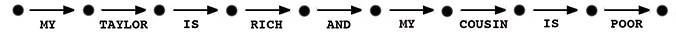
\includegraphics{Figure(1a).jpg}\nonumber
\end{equation}
{\bf{(1b)}} The kind $\underset{\raisebox{0.4ex}{$\scriptstyle \rightarrow $}}{\mathcal{L}}^{\rotatebox[origin=c]{-180}{$\circlearrowright$}}$ of one-way linear sentences with (possible) loops, e.g.,
\begin{equation}
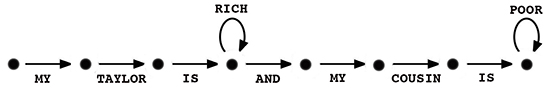
\includegraphics{Figure(1b).jpg}\nonumber
\end{equation}
{\bf{(2a)}} The kind $\underset{\rightleftarrows}{\mathcal{L}}$ of two-way linear sentences without loops, e.g.,
\begin{equation}
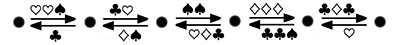
\includegraphics{Figure(2a).jpg}\nonumber
\end{equation}
{\bf{(2b)}} The kind $\underset{\rightleftarrows}{\mathcal{L}}^{\rotatebox[origin=c]{-180}{$\circlearrowright$}}$ of two-way linear sentences with (possible) loops, e.g.,
\begin{equation}
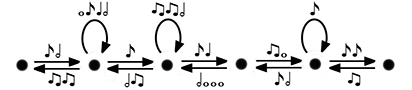
\includegraphics{Figure(2b).jpg}\nonumber
\end{equation}

\noindent the alphabets being the standard (cap) 26-letter alphabet,  $\{$ {\boldmath ${\heartsuit, \diamondsuit,  \clubsuit, \spadesuit}$} $\}$, $\{$ {\boldmath ${\eighthnote,\halfnote,\twonotes,\fullnote,\quarternote}$} $\}$.\\

\noindent The finite alphabet $\mathbb{A}$ can be an arbitrary set of symbols and the words put on arrows or loops are mathematical words, i.e., arbitrary finite sequences of ``letters" in $\mathbb{A}$. Graphical sentences can be used to encode sets of sentences in a compact way: the \emph{readable sentences} being the sequences of words corresponding to directed paths in the graph, the letters of each word being read from source to target of its corresponding arrow or loop.\\

\noindent For example, the following are readable sentences\\

\noindent Kind $\underset{\raisebox{0.4ex}{$\scriptstyle \rightarrow $}}{\mathcal{L}}$ : \,\,``\,{\texttt{\textbf{MY COUSIN IS POOR}}}''.\\
Kind $\underset{\raisebox{0.4ex}{$\scriptstyle \rightarrow $}}{\mathcal{L}}^{\rotatebox[origin=c]{-180}{$\circlearrowright$}}$ : ``\,{\texttt{\textbf{MY TAYLOR IS RICH RICH RICH AND MY COUSIN IS POOR POOR}}}''.\\
Kind $\underset{\rightleftarrows}{\mathcal{L}}$ : \,\,\,\,``$\clubsuit  \heartsuit \, \,\,   \spadesuit \diamondsuit \,\,\, \clubsuit  \heartsuit \,\,\, \spadesuit \spadesuit \,\,\, \diamondsuit \diamondsuit \diamondsuit \,\,\, \spadesuit \spadesuit  \spadesuit \,\,\,\clubsuit \diamondsuit \heartsuit $''.\\
Kind $\underset{\rightleftarrows}{\mathcal{L}}^{\rotatebox[origin=c]{-180}{$\circlearrowright$}}$ :  ``$\fullnote \eighthnote \quarternote \halfnote \,\,\, \eighthnote \,\,\, \twonotes  \halfnote \,\,\, \eighthnote \,\,\, \twonotes \twonotes \halfnote \,\,\, \eighthnote \quarternote \,\,\,  \twonotes \fullnote \,\,\, \halfnote \eighthnote \,\,\,  \fullnote \fullnote \fullnote \halfnote$\,''.\\

\noindent A family of parameters can be associated to each graphical sentence : the number of occurrences of each letter, the number of words, of loops, of arrows, etc. 
\\

\noindent {\bf{THE CLASSROOM  ACTIVITY.}} After introducing the above kinds of graphical sentences, the teacher can then ask the following question :\\

\noindent {\bf{Q}} : {\it{How many graphical sentences of kind $\underset{\raisebox{0.4ex}{$\scriptstyle \rightarrow $}}{\mathcal{L}}^{\rotatebox[origin=c]{-180}{$\circlearrowright$}}$  contain exactly $5$ arrows, $3$ loops, $5$ times letter A, $4$ times letter C, $5$ times letter G and $6$ times letter T and no other letter}} {\bf{?}}\\

\noindent $\bullet$ STEP 1. In order to take into account the values of these parameters in a compact way, suggest the student to give a {\emph{weight}} to each graphical sentence in the form of a monomial in the symbolic variables $``\uparrow"$, ${\rotatebox[origin=c]{-180}{$\circlearrowright$}}"$, and each letter $``a"$ of alphabet $\mathbb{A}$. The weight ${\bf{w}}s$ of the following graphical sentence $s$ of kind $\underset{\raisebox{0.4ex}{$\scriptstyle \rightarrow $}}{\mathcal{L}}^{\rotatebox[origin=c]{-180}{$\circlearrowright$}}$  
\begin{equation}
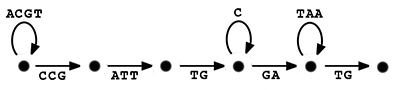
\includegraphics{ACGT.jpg}\nonumber
\end{equation}
would be
\begin{equation}\label{weight}
\text{weight}(s) = {\bf{w}}s=\uparrow^{5} \!{\rotatebox[origin=c]{-180}{$\circlearrowright$}}^3A^5C^4G^5T^6 
\end{equation}
where the exponent of each symbolic variable is the number of occurrences it appears in $s$ (exponent $0$ means that the corresponding item does not appear in $s$). Of course, the weight of a graphical sentence of kinds $\underset{\raisebox{0.4ex}{$\scriptstyle \rightarrow $}}{\mathcal{L}}$ and $\underset{\rightleftarrows}{\mathcal{L}}$ will never contain the variable $``{\rotatebox[origin=c]{-180}{$\circlearrowright$}}"$. \\

\noindent $\bullet$ STEP 2. Define the weight ${\bf{w}}\mathcal{K}$ (or inventory) of any kind $\mathcal{K}$ of graphical sentences as the formal sum of weight of its elements:
\begin{equation}\label{inv}
\text{inventory}(\mathcal{K})={\bf{w}}\mathcal{K}=\sum_{s \in{\mathcal{K}}}{\bf{w}}s
\end{equation}
and convice the students that the answer to question {\bf{Q}} is the coefficient of monomial (\ref{weight}) after collecting similar terms in the inventory ${\bf{w}}\underset{\raisebox{0.4ex}{$\scriptstyle \rightarrow $}}{\mathcal{L}}^{\rotatebox[origin=c]{-180}{$\circlearrowright$}}$  of the kind $\underset{\raisebox{0.4ex}{$\scriptstyle \rightarrow $}}{\mathcal{L}}^{\rotatebox[origin=c]{-180}{$\circlearrowright$}}$  of graphical sentences.\\

\noindent $\bullet$ STEP 3. Help students to find closed forms for the inventories ${\bf{w}}\underset{\raisebox{0.4ex}{$\scriptstyle \rightarrow $}}{\mathcal{L}}$ and ${\bf{w}}\underset{\raisebox{0.4ex}{$\scriptstyle \rightarrow $}}{\mathcal{L}}^{\rotatebox[origin=c]{-180}{$\circlearrowright$}}$ by making use, among other things, of the geometric series
\begin{equation}
\frac{1}{1-X} = 1+X+X^2+X^3+\cdots,
\end{equation}
and suggest to use the CA system to answer question {\bf{Q}}. Of course, when using the CA system, it is more convenient to use other symbols for the variables : for example, $\alpha$ instead of $\uparrow$, $\lambda$ instead of ${\rotatebox[origin=c]{-180}{$\circlearrowright$}}$ and $a_1,a_2, \dots, a_n$ for the letters of alphabet $\mathbb{A}$. \\

\noindent $\bullet$ STEP 4. The teacher goes one step further by challenging students to compute the inventories of the kinds $\underset{\rightleftarrows}{\mathcal{L}}$ and  $\underset{\rightleftarrows}{\mathcal{L}}^{\rotatebox[origin=c]{-180}{$\circlearrowright$}}$ of {\emph{{\underline{two-way}} linear graphical sentences}}. The extra difficulty is to be careful to ``count'' only once those kind of graphical sentences having a $180^\circ$ symmetry.\\

\noindent $\bullet$ STEP 5. Manipulate inventories (by assigning values to variables, making some variables equal, differentiating with respect to some variables, etc) in order to extract more information on the kind of graphical sentences under study.\\

\noindent By the above activity, the students will learn the following facts :\\

\noindent $\bullet$ Geometric (and power) series do not need to be convergent in order to be useful.\\
$\bullet$ Any symbol can be interpreted as an algebraic variable in concrete situations.\\
$\bullet$ Monomials can help in making various kinds of ``inventories" in classes of objects.\\
$\bullet$ Manipulation of inventories give much information on various kinds of objects.\\
$\bullet$ Computer algebra can be of great help even in ``simple" enumerative questions.\\

\KEYWORDS {Graphs, sentences, graphical sentences, generating functions.}\\

\noindent{\bf{MSC2010 Classification}}: {05A15, 05C30}

\begin{thebibliography}{9}

\bibitem{LabLaf} \textsc{G. Labelle; L. Laforest}, A Combinatorial Analysis of Tree-Like Sentences.
\emph{Open Journal of Discrete Mathematics} \textbf{volume}(5), 32--53  (2015).

\end{thebibliography}

\vspace{1cm}

% Full Affiliation of all authors
\ADDRESS{1}{
D\'ep. de math\'ematiques + LaCIM  \\U. du Qu\'ebec \`a Montr\'eal (UQAM) \\
C.P. 8888, Succ. Centre-ville, \\
Montr\'eal (Qu\'ebec) Canada H3C 3P8\\
\texttt{labelle.gilbert@uqam.ca}
}

\vspace{.5cm}

\ADDRESS{2}{
D\'ep. d'informatique + LaCIM  \\U. du Qu\'ebec \`a Montr\'eal (UQAM) \\
C.P. 8888, Succ. Centre-ville, \\
Montr\'eal (Qu\'ebec) Canada H3C 3P8\\
\texttt{laforest.louise@uqam.ca}
}


\end{document}
